\documentclass{article}
	\usepackage{geometry}
	\usepackage{graphicx}
	\usepackage{indentfirst}
	\usepackage[hyphens]{url}
	\usepackage{listings}
	\usepackage{color}
	\definecolor{gray}{rgb}{0.3,0.3,0.3}
	\usepackage{caption}
	\DeclareCaptionFont{white}{\color{white}}
	\DeclareCaptionFormat{listing}{\colorbox{gray}{\parbox{\textwidth}{#1#2#3}}}
	\captionsetup[lstlisting]{format=listing,labelfont={bf,sf,white},textfont={bf,sf,white}}
	\usepackage{xcolor}
	\usepackage{booktabs}
	\captionsetup[table]{labelfont=bf}
	\usepackage[colorlinks,linkcolor=red]{hyperref}

	\begin{document}
		\begin{center}\textbf{Bo Zhang\\01063214}
		\end{center}
		\section{Karate Club Split Prediction}
		We know the result of the Karate Club (Zachary, 1977) split. Prove or disprove that the result of split could have been predicted by the weighted graph of social interactions. How well does the mathematical model represent reality?\\

		\noindent\textbf{Algorithm: }\\
		\indent1. Use the package ``igraphml''(\url{http://igraph.org/r/}) to analyze.\\
		\indent2. Load the graph data.\\
		\indent3. Use the edge betweenness community detection algorithm.\\
		\indent4. Cut the merge tree to get 2 communities.\\
		\indent5. Plot the 2 communities.\\

		\noindent\textbf{Source code:}
		\lstinputlisting[language=R, breakatwhitespace=false), label=Q1.R, caption=The content of Q1.R]{Q1.R}

		\noindent\\\textbf{Results:}
		\begin{figure}[!htb]
			\centering 
			\href{https://github.com/zhangboroy/cs532-s17/blob/master/assg05_submission/group2.png}
			{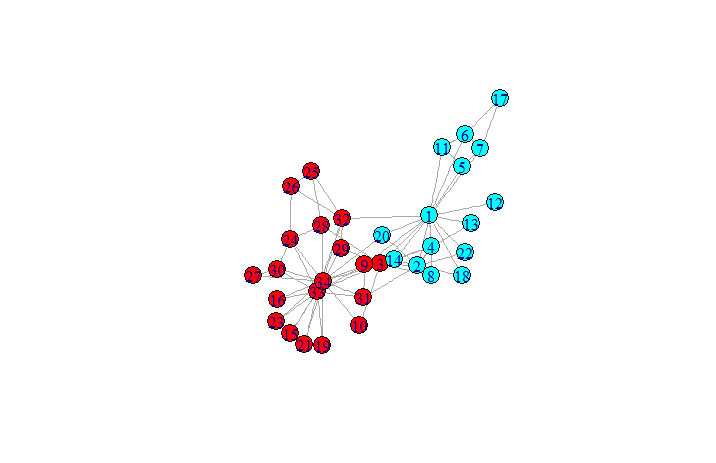
\includegraphics[width=0.39\textwidth]{group2.png}}
			\label{fig:Prediction of Karate Club Splits into 2 Groups}
			\caption{Prediction of Karate Club Splits into 2 Groups}
		\end{figure}

		\begin{table}[!htb]
			\centering
			\caption{\textbf{Edge Betweenness Algorithm Result}}
			\begin{tabular}{cccc}
				\toprule
				\textbf{Individual Number} & \textbf{Actual Club After Split} & \textbf{Predicted Club After Split} & \textbf{Hit/Miss}\\
				\midrule
				1 & 2 & 2 & Hit\\
				2 & 2 & 2 & Hit\\
				3 & 2 & 1 & Miss\\
				4 & 2 & 2 & Hit\\
				5 & 2 & 2 & Hit\\
				6 & 2 & 2 & Hit\\
				7 & 2 & 2 & Hit\\
				8 & 2 & 2 & Hit\\
				9 & 2 & 1 & Miss\\
				10 & 1 & 1 & Hit\\
				11 & 2 & 2 & Hit\\
				12 & 2 & 2 & Hit\\
				13 & 2 & 2 & Hit\\
				14 & 2 & 2 & Hit\\
				15 & 1 & 1 & Hit\\
				16 & 1 & 1 & Hit\\
				17 & 2 & 2 & Hit\\
				18 & 2 & 2 & Hit\\
				19 & 1 & 1 & Hit\\
				20 & 2 & 2 & Hit\\
				21 & 1 & 1 & Hit\\
				22 & 2 & 2 & Hit\\
				23 & 1 & 1 & Hit\\
				24 & 1 & 1 & Hit\\
				25 & 1 & 1 & Hit\\
				26 & 1 & 1 & Hit\\
				27 & 1 & 1 & Hit\\
				28 & 1 & 1 & Hit\\
				29 & 1 & 1 & Hit\\
				30 & 1 & 1 & Hit\\
				31 & 1 & 1 & Hit\\
				32 & 1 & 1 & Hit\\
				33 & 1 & 1 & Hit\\
				34 & 1 & 1 & Hit\\
				\bottomrule
			\end{tabular}
		\end{table}

		According to these figures, 32(94\%) hits and 2(6\%) misses. So the result of split could have been predicted by the weighted graph of social interactions. And the accuracy of the mathematical model is 94\% based on this case.\\
		\section{Karate Club Splits into Groups of 3, 4 and 5}
		\indent We know the group split in two different groups. Suppose the disagreements in the group were more nuanced -- what would the clubs look like if they split into groups of 3, 4, and 5?\\\\
		\textbf{Algorithm:}\\
		\indent1. Use the package ``igraphml''(\url{http://igraph.org/r/}) to analyze.\\
		\indent2. Load the graph data.\\
		\indent3. Use the edge betweenness community detection algorithm.\\
		\indent4. Cut the merge tree to get 3 communities.\\
		\indent5. Plot the 3 communities.\\
		\indent4. Cut the merge tree to get 4 communities.\\
		\indent5. Plot the 4 communities.\\
		\indent4. Cut the merge tree to get 5 communities.\\
		\indent5. Plot the 5 communities.\\

		\noindent\textbf{Source code:}
		\lstinputlisting[language=R, breakatwhitespace=false), label=Q2.R, caption=The content of Q2.R]{Q2.R}

		\noindent\\\textbf{Results: }
		\begin{figure}[!htb]
			\centering
			\href{https://github.com/zhangboroy/cs532-s17/blob/master/assg05_submission/group3.png}
			{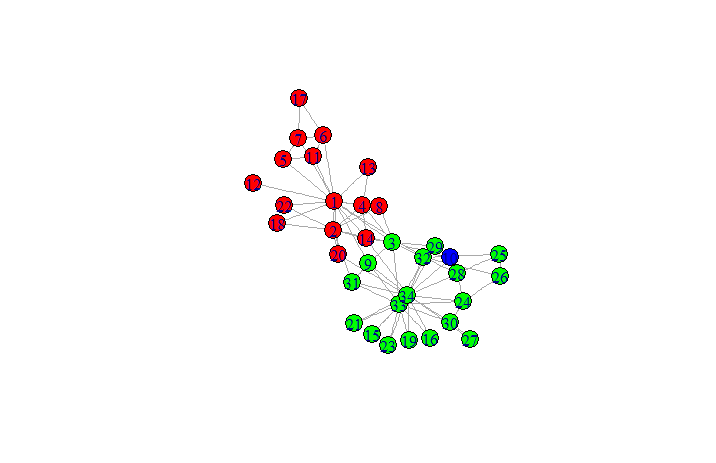
\includegraphics[width=0.37\textwidth]{group3.png}}
			\label{fig:Prediction of Karate Club Splits into 3 Groups}
			\caption{Prediction of Karate Club Splits into 3 Groups}
			\href{https://github.com/zhangboroy/cs532-s17/blob/master/assg05_submission/group4.png}
			{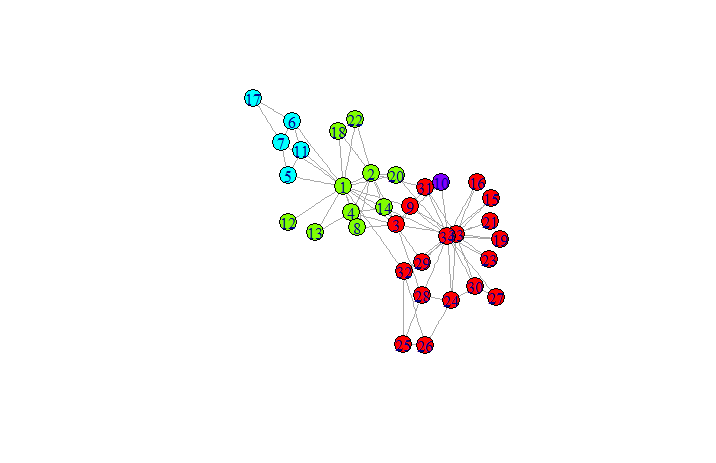
\includegraphics[width=0.37\textwidth]{group4.png}}
			\label{fig:Prediction of Karate Club Splits into 4 Groups}
			\caption{Prediction of Karate Club Splits into 4 Groups}
			\href{https://github.com/zhangboroy/cs532-s17/blob/master/assg05_submission/group5.png}
			{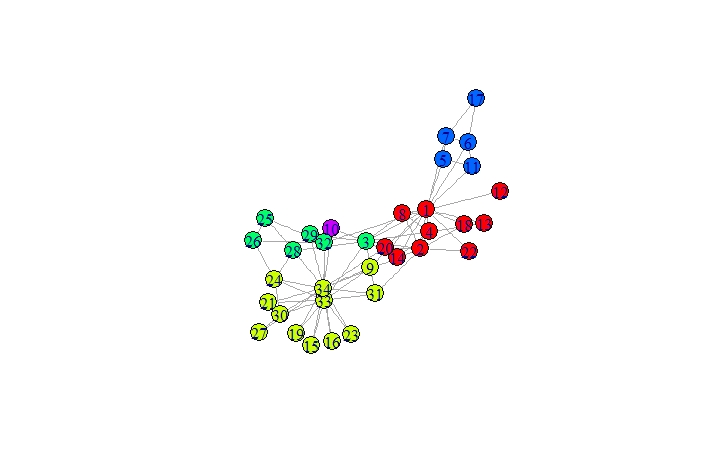
\includegraphics[width=0.37\textwidth]{group5.png}}
			\label{fig:Prediction of Karate Club Splits into 5 Groups}
			\caption{Prediction of Karate Club Splits into 5 Groups}
		\end{figure}
	\end{document}